\chapter{Luminosity  Measurement and Calibration}
\label{ch3}

Accurately measuring the luminosity delivered to the CMS experiment by the LHC is essential for various reasons. Online, the luminosity measurement provides feedback on the LHC and CMS performance and operations, including measuring trigger rates. In offline analysis, the luminosity measurement is a critical component for measuring the cross-section of observed processes or setting upper limits in searches for processes beyond the standard model.

As we see, to measure luminosity, a total of seven luminometers are used at CMS, and each of them reads out a specific quantity observed in the detector, such as hits, tracks, or clusters. The rate R measured by the luminometer is proportional to the instantaneous luminosity, $\mathcal{L}_{inst}$, with the constant of proportionality given by the visible cross-section $\sigma{vis}$ \cite{pas_18}.

\begin{equation}
R(t)=\mathcal{L}_{inst}\sigma_{vis}
\label{lumi_exp_gen}
\end{equation}

The determination of $\sigma_{vis}$ is performed through van der Meer (vdM) scans using a specialized LHC machine setup. This chapter provides a description of this procedure, specifically applied with the PCC method. Additionally, the selection of stable "good" modules necessary for precise luminosity measurements will also be discussed.

\section{Pixel Cluster Counting method}

The PCC method utilizes the rate of pixel clusters in the CMS silicon pixel detector to determine an offline luminosity measurement, this method exploits the very large number of pixels in the inner part of the CMS tracking system,it means that the probability of a given pixel being hit by two different charged particles from the same bunch crossing is exceedingly small, this large area and low occupancy yield measurements with excellent linear response with the pile-up (number of interactions per bunch crossing)$\mu$ \citep{lumi_precise_2015_2016}, therefore an accurate measure of instantaneous luminosity with a high statistical precision.\\

However, the statistical precision for a single 23-second period or "luminosity section" is not as high as for online luminometers due to the limited CMS trigger bandwidth available for collecting data. Nonetheless, over longer time periods, this method provides a stable and highly precise luminosity measurement. On average, the detector occupancy is less than 0.1\% \cite{pas_18}.\\

Figure  \ref{pileup} shows a simulation made in 2016 with a representative PCC distribution at $\mu$ = 45 and the average PCC as a function of $\mu$. The latter distribution is fitted with a first-order polynomial, assuming no correlations among different values of $\mu$. Good agreement is seen based on the estimated goodness-of-fit $\chi^{2}$ per degree of freedom (dof) value of about 0.5 , indicating linearity under simulated conditions \cite{lumi_precise_2015_2016}.

\begin{center}
  \begin{figure}[h!]
    \centering
    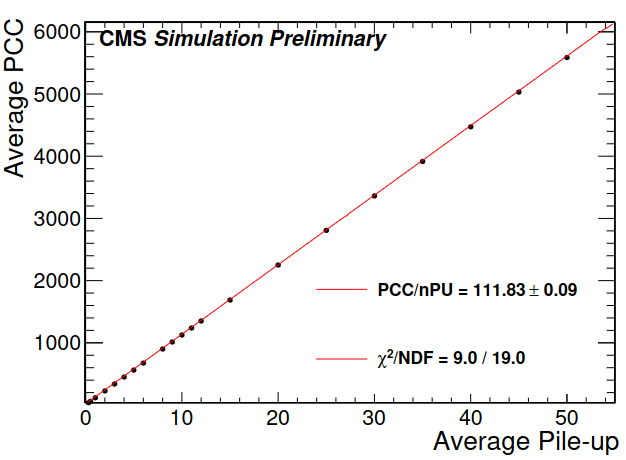
\includegraphics[scale=.3]{Chapter3/pileup_lineality.png} 
    \caption[Linearity with pile-up]{ The left plot shows the number of pixel clusters and their statistical uncertainty from simulation of pileup following a Poisson distribution with a mean of 45. The right plot shows the mean number of pixel clusters from simulation as a function of mean pileup. The red curve is a first-order polynomial fit with slope and $\chi^{2}/ndof$ values shown in the legend. The lower panel of the right plot shows the difference between the simulation and the linear fit in black points. The green band is the final linearity uncertainty for the 2016 data set \cite{lumi_precise_2015_2016} }
    \label{pileup}
  \end{figure}
\end{center}

To obtain the mean number of pixel clusters per event, several zero-bias events are averaged. This value is given by :

\begin{equation}
\left < N_{\text{cluster}} \right > = \left < N_{\text{pixel}/\text{interaction}} \right >  \left < N_{\text{interactions}} \right > \equiv \left < N_{\text{pixel}/\text{interaction}} \right > \mu
\end{equation}

where $\mu$ is the average number of interactions per bunch crossing and is refered as pileup \cite{PCC_PAS_12_001}. Under minimum bias conditions, $\mu$ can be expressed as: 

\begin{equation}
\mu = \frac{\sigma_{\text{minBias}}}{f} \cdot \mathcal{L}_{inst}
\end{equation}

where $f$ is the LHC revolution frequency and $\mathcal{L}_{inst}$ is the single bunch instantaneous luminosity (SBIL). The minimum bias cross section here is related to the PCC visible cross section by the mean number of clusters per interaction:

\begin{equation}
\sigma_{vis}^{PCC}= \left < N_{\text{pixel}/\text{interaction}} \right >\cdot \sigma_{\text{minBias}}
\end{equation}

Combining everything, the PCC luminosity measurement is obtained as:

\begin{equation}
\mathcal{L}_{inst}=\frac{\left < N_{\text{cluster}} \right >}{\sigma_{vis}^{PCC}} \cdot f
\end{equation}

In the PCC measurement, the innermost layer of the pixel detector is excluded from the analysis due to significant dynamic inefficiency effects \cite{pas_18}. At higher $\mathcal{L}_{inst}$, the hit efficiency in this layer decreases because the readout chip cannot process all of the hits. Only modules that consistently perform well for luminosity purposes throughout the year are utilized in the measurement.

For the VdM measurement, a special trigger mode is employed, which enables a higher data rate for PCC to acquire the required statistical precision. However, this mode is only active for five bunch crossings, and data are taken exclusively during this period.

\section{Luminosity calibration: van der Meer method}

As discussed in Chapter 1, the instantaneous luminosity for a single colliding bunch is described by Eq. (\ref{luminosity_2}). In practice, while the measurement of the beam currents $N_{1,2}$ is well determined, the individual proton density functions cannot be directly measured. To address this, the VdM method involves a specific machine setup that allows for the determination of the two beam overlap integrals. This is achieved by varying the separation between the beams and measuring the resulting rates, which can be used to obtain density profiles that are close to normal distributions.

\begin{equation}
\int \rho_{x1}(x) \rho_{x2}(x) dx = \frac{R_{x}(0)}{\int R_{x}(\Delta) d\Delta}
\end{equation}

where $R_{x}(\Delta)$ is the rate measured when the two beams are separated in $x$ by a distance $\Delta$; a asimilar equation can be written in $y$. Then the beam overlap width $\Sigma_{x}$ (and similarly $\Sigma_{y}$) is defined as \cite{pas_18}:

\begin{equation}
\Sigma_{x}= \frac{1}{\sqrt{2\pi}} \frac{\int R_{x}(\Delta)d\Delta}{R_{x}(0)}
\label{CapSigma}
\end{equation}

This process leads to the final expression for luminosity for a single colliding bunch:

\begin{equation}
\mathcal{L}_{inst}=\frac{N_{1} N_{2}f}{2 \pi \Sigma_{x}\Sigma_{y}}
\end{equation}

where $N_{1,2}$ are the particles per bunch (bunch current) and  $f= 11246$ Hz is the bunch orbit frequency around the LHC ring.\\

Therefore, the formula used to measure the visible cross sections $\sigma_{vis}$ takes the following form:

\begin{equation}
  \sigma_{vis}=\frac{2\pi \Sigma_{x} \Sigma_{y} R(0, 0)}{N_{1}N_{2} f}
  \label{sigmavis_eq}
\end{equation}

Experimentally, the quantities $\Sigma_{x}$ and $\Sigma_{y}$, as defined in Eq. (\ref{CapSigma}), are determined by conducting two separate scans in the $x$ and $y$ directions, respectively. These scans are performed by varying the separation between the beams in each direction and measuring the rate $R(0,0)$, which is normalized by the product of the beam currents, at a fixed number of separation steps. The separation steps are determined through curve fitting of the scan data based on the luminometer rate measurements obtained during the vdM scans. While the beam widths are the same for all luminometers, the peaks of the corresponding scan curves are luminometer-specific. Figure \ref{vdm_sketch} depicts a schematic of the beam positions during vdM scans in the $x$ and $y$ planes, along with the detector rate as a function of beam separation  \cite{pas_18}.

Only modules that are found to operate consistently well for luminosity purposes during the year of the VdM scan are used in the measurement.  

\begin{center}
  \begin{figure}[h!]
    \centering
    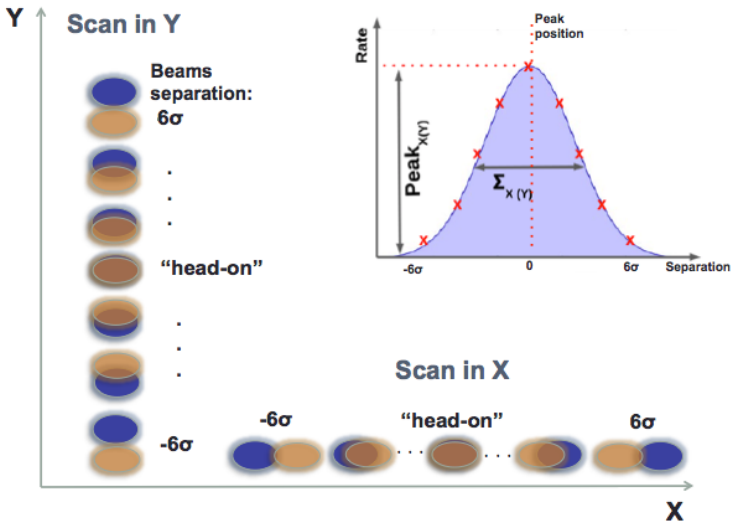
\includegraphics[scale=.37]{Chapter3/vdm_sketch.png}
    \caption[Sketch of a vdM scan in x and y planes and example of fitting resulting rates]{ The sketch of a vdM scan in $x$ and $y$ planes. The indent sketch is an example of the fitting of the resulting rates \cite{vdM_sketch}.}
    \label{vdm_sketch}
  \end{figure}
\end{center}


\section{Module selection}

To ensure accurate luminosity measurement, a veto list is created to remove any modules exhibiting long-term performance variations, indicating a non-physical shift in their cluster counts. With a total of 1856 modules in the pixel system, all of them can be considered in the luminosity measurement; however, non-zero occupancy and non-linear effects can pose challenges for accurate measurement. Thus, to identify "good" and "stable" modules, a subset is selected by eliminating  underperforming or "bad" modules and comparing their relative contributions to the cross section. Those with relatively consistent contributions across standard physics runs are kept, while those with significant changes in their relative cross section compared to the averaged relative contribution are rejected. The Module selection is made as:

\begin{itemize}
\item Poor statistics lumisections are removed by applying selection on total PCC.
\item Barrel layer-1 modules are removed, as these modules are significantly affected by dynamic inefficiency.
\item A loose selection of 7\% based on RMS/mean of module weight is applied. Modules with significantly large RMS/mean are removed with this selection as shown in \ref{goodmodule}.
\item The module stability is re-evaluated based on RMS/mean values using an iterative method where appropriate selections are applied to remove underperforming modules until a stable luminosity is attained.
\end{itemize}

\begin{center}
  \begin{figure}[h!]
    \centering
    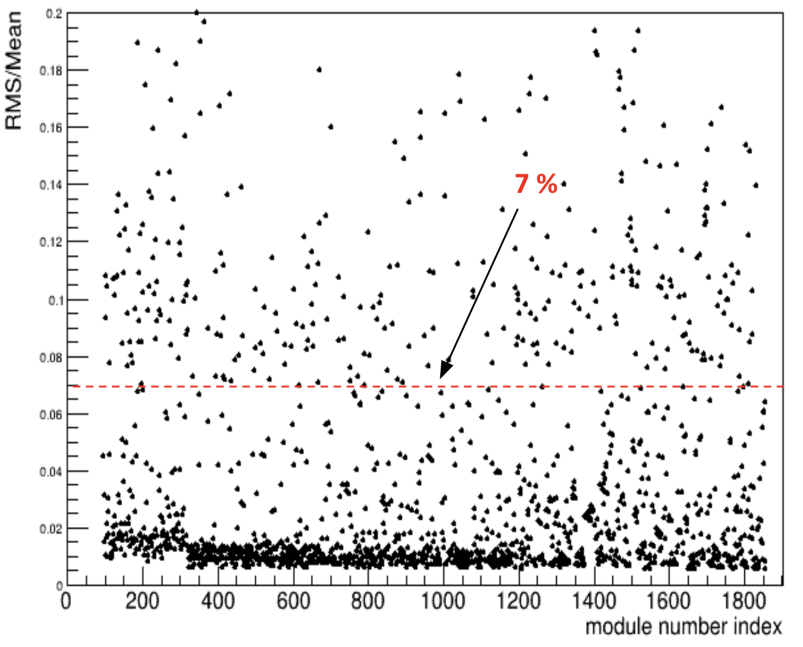
\includegraphics[scale=.20]{Chapter4/RMSmean.png}
    \caption[RMS/mean Module  Stability]{ RMS/mean values of module weight for all pixel modules. Each pixel module is represented by a module number index.} 
    \label{goodmodule}
  \end{figure}
\end{center}

To ensure accurate measurements, a pixel module veto list is established for each period, recognizing that different periods may have varying numbers of well-performing modules. The pixel detector is subject to changing conditions over time, such as detector noise, aging effects, and radiation damage. Stability of the pixel modules is assessed based on changes in the module PCC ratio relative to the total PCC, known as module weight. These variations are evaluated over an interval of 23 seconds, corresponding to the granularity of the luminosity database. The pixel module veto list is first generated for the period 2022F containing the vdM fill and subsequently for the periods ,C, D, E and G,  following the same procedure.  


To further improve the stability of the PCC measurement, a 4\% RMS common module vetolist is created as shown in table \ref{common  veto module}. The approach to derive the common module veto list is to start by combining module vetolists of period C and D; then combine C, D and E; and so on. The zero-bias PCC data is reprocessed using this common module vetolist. 

\begin{table}[ht]
\centering
\caption{Number of good and bad modules for the combined vetolist, after each iteration of the 4\% RMS selection with an additional period.}
\begin{tabular}{ccc}
\textbf{Period} & \textbf{\# bad modules} & \textbf{\# good modules}  \\ 
\toprule
2022C+D         & 886                     & 970                       \\
2022C+D+E       & 1106                    & 750                       \\
2022C+D+E+F     & 1307                    & 549                       \\
2022C+D+E+F+G   & 1411                    & 445                   
\label{common  veto module}   
\end{tabular}
\end{table}

\noindent This final common veto in conjunction with background subtraction  is used for the last reprocesing data analysed with the VdM scan. 